% Options for packages loaded elsewhere
\PassOptionsToPackage{unicode}{hyperref}
\PassOptionsToPackage{hyphens}{url}
%
\documentclass[
]{article}
\usepackage{amsmath,amssymb}
\usepackage{lmodern}
\usepackage{ifxetex,ifluatex}
\ifnum 0\ifxetex 1\fi\ifluatex 1\fi=0 % if pdftex
  \usepackage[T1]{fontenc}
  \usepackage[utf8]{inputenc}
  \usepackage{textcomp} % provide euro and other symbols
\else % if luatex or xetex
  \usepackage{unicode-math}
  \defaultfontfeatures{Scale=MatchLowercase}
  \defaultfontfeatures[\rmfamily]{Ligatures=TeX,Scale=1}
\fi
% Use upquote if available, for straight quotes in verbatim environments
\IfFileExists{upquote.sty}{\usepackage{upquote}}{}
\IfFileExists{microtype.sty}{% use microtype if available
  \usepackage[]{microtype}
  \UseMicrotypeSet[protrusion]{basicmath} % disable protrusion for tt fonts
}{}
\makeatletter
\@ifundefined{KOMAClassName}{% if non-KOMA class
  \IfFileExists{parskip.sty}{%
    \usepackage{parskip}
  }{% else
    \setlength{\parindent}{0pt}
    \setlength{\parskip}{6pt plus 2pt minus 1pt}}
}{% if KOMA class
  \KOMAoptions{parskip=half}}
\makeatother
\usepackage{xcolor}
\IfFileExists{xurl.sty}{\usepackage{xurl}}{} % add URL line breaks if available
\IfFileExists{bookmark.sty}{\usepackage{bookmark}}{\usepackage{hyperref}}
\hypersetup{
  pdftitle={Super Bowl Ads},
  pdfauthor={MGinorio},
  hidelinks,
  pdfcreator={LaTeX via pandoc}}
\urlstyle{same} % disable monospaced font for URLs
\usepackage[margin=1in]{geometry}
\usepackage{color}
\usepackage{fancyvrb}
\newcommand{\VerbBar}{|}
\newcommand{\VERB}{\Verb[commandchars=\\\{\}]}
\DefineVerbatimEnvironment{Highlighting}{Verbatim}{commandchars=\\\{\}}
% Add ',fontsize=\small' for more characters per line
\usepackage{framed}
\definecolor{shadecolor}{RGB}{248,248,248}
\newenvironment{Shaded}{\begin{snugshade}}{\end{snugshade}}
\newcommand{\AlertTok}[1]{\textcolor[rgb]{0.94,0.16,0.16}{#1}}
\newcommand{\AnnotationTok}[1]{\textcolor[rgb]{0.56,0.35,0.01}{\textbf{\textit{#1}}}}
\newcommand{\AttributeTok}[1]{\textcolor[rgb]{0.77,0.63,0.00}{#1}}
\newcommand{\BaseNTok}[1]{\textcolor[rgb]{0.00,0.00,0.81}{#1}}
\newcommand{\BuiltInTok}[1]{#1}
\newcommand{\CharTok}[1]{\textcolor[rgb]{0.31,0.60,0.02}{#1}}
\newcommand{\CommentTok}[1]{\textcolor[rgb]{0.56,0.35,0.01}{\textit{#1}}}
\newcommand{\CommentVarTok}[1]{\textcolor[rgb]{0.56,0.35,0.01}{\textbf{\textit{#1}}}}
\newcommand{\ConstantTok}[1]{\textcolor[rgb]{0.00,0.00,0.00}{#1}}
\newcommand{\ControlFlowTok}[1]{\textcolor[rgb]{0.13,0.29,0.53}{\textbf{#1}}}
\newcommand{\DataTypeTok}[1]{\textcolor[rgb]{0.13,0.29,0.53}{#1}}
\newcommand{\DecValTok}[1]{\textcolor[rgb]{0.00,0.00,0.81}{#1}}
\newcommand{\DocumentationTok}[1]{\textcolor[rgb]{0.56,0.35,0.01}{\textbf{\textit{#1}}}}
\newcommand{\ErrorTok}[1]{\textcolor[rgb]{0.64,0.00,0.00}{\textbf{#1}}}
\newcommand{\ExtensionTok}[1]{#1}
\newcommand{\FloatTok}[1]{\textcolor[rgb]{0.00,0.00,0.81}{#1}}
\newcommand{\FunctionTok}[1]{\textcolor[rgb]{0.00,0.00,0.00}{#1}}
\newcommand{\ImportTok}[1]{#1}
\newcommand{\InformationTok}[1]{\textcolor[rgb]{0.56,0.35,0.01}{\textbf{\textit{#1}}}}
\newcommand{\KeywordTok}[1]{\textcolor[rgb]{0.13,0.29,0.53}{\textbf{#1}}}
\newcommand{\NormalTok}[1]{#1}
\newcommand{\OperatorTok}[1]{\textcolor[rgb]{0.81,0.36,0.00}{\textbf{#1}}}
\newcommand{\OtherTok}[1]{\textcolor[rgb]{0.56,0.35,0.01}{#1}}
\newcommand{\PreprocessorTok}[1]{\textcolor[rgb]{0.56,0.35,0.01}{\textit{#1}}}
\newcommand{\RegionMarkerTok}[1]{#1}
\newcommand{\SpecialCharTok}[1]{\textcolor[rgb]{0.00,0.00,0.00}{#1}}
\newcommand{\SpecialStringTok}[1]{\textcolor[rgb]{0.31,0.60,0.02}{#1}}
\newcommand{\StringTok}[1]{\textcolor[rgb]{0.31,0.60,0.02}{#1}}
\newcommand{\VariableTok}[1]{\textcolor[rgb]{0.00,0.00,0.00}{#1}}
\newcommand{\VerbatimStringTok}[1]{\textcolor[rgb]{0.31,0.60,0.02}{#1}}
\newcommand{\WarningTok}[1]{\textcolor[rgb]{0.56,0.35,0.01}{\textbf{\textit{#1}}}}
\usepackage{graphicx}
\makeatletter
\def\maxwidth{\ifdim\Gin@nat@width>\linewidth\linewidth\else\Gin@nat@width\fi}
\def\maxheight{\ifdim\Gin@nat@height>\textheight\textheight\else\Gin@nat@height\fi}
\makeatother
% Scale images if necessary, so that they will not overflow the page
% margins by default, and it is still possible to overwrite the defaults
% using explicit options in \includegraphics[width, height, ...]{}
\setkeys{Gin}{width=\maxwidth,height=\maxheight,keepaspectratio}
% Set default figure placement to htbp
\makeatletter
\def\fps@figure{htbp}
\makeatother
\setlength{\emergencystretch}{3em} % prevent overfull lines
\providecommand{\tightlist}{%
  \setlength{\itemsep}{0pt}\setlength{\parskip}{0pt}}
\setcounter{secnumdepth}{-\maxdimen} % remove section numbering
\ifluatex
  \usepackage{selnolig}  % disable illegal ligatures
\fi

\title{Super Bowl Ads}
\author{MGinorio}
\date{}

\begin{document}
\maketitle

\hypertarget{super-bowl-analysis}{%
\subsection{Super Bowl Analysis}\label{super-bowl-analysis}}

\hypertarget{the-american-super-bowl-is-a-statement-in-the-advertisement-industry-due-to-the-creative-nature-of-their-ads.-every-year-many-brands-showcase-their-best-pieces-of-advertisement-and-see-which-team-did-it-better}{%
\paragraph{The American Super Bowl is a statement in the Advertisement
industry due to the creative nature of their ads. Every year many brands
showcase their best pieces of advertisement and see which team did it
better}\label{the-american-super-bowl-is-a-statement-in-the-advertisement-industry-due-to-the-creative-nature-of-their-ads.-every-year-many-brands-showcase-their-best-pieces-of-advertisement-and-see-which-team-did-it-better}}

\hypertarget{this-time-we-are-asking-the-question---what-is-behind-the-creation-of-the-ads-was-it-funny-did-it-use-sex-to-sell-the-product-did-it-feature-a-celebrity}{%
\paragraph{This time we are asking the question - what is behind the
creation of the ads? Was it funny? did it use sex to sell the product?
did it feature a
celebrity?}\label{this-time-we-are-asking-the-question---what-is-behind-the-creation-of-the-ads-was-it-funny-did-it-use-sex-to-sell-the-product-did-it-feature-a-celebrity}}

\hypertarget{problem-statement}{%
\subsection{Problem Statement}\label{problem-statement}}

\hypertarget{the-aim-of-this-analysis-is-to-determine-which-category-predominates-in-the-super-bowl-add-arena.-is-it-sex-comedy-animals-or-celebrities}{%
\paragraph{The aim of this analysis is to determine which category
predominates in the super bowl add arena. Is it sex, comedy, animals or
celebrities?}\label{the-aim-of-this-analysis-is-to-determine-which-category-predominates-in-the-super-bowl-add-arena.-is-it-sex-comedy-animals-or-celebrities}}

\hypertarget{implementation}{%
\subsection{Implementation}\label{implementation}}

\hypertarget{the-data-was-scraped-and-manipulated-accordingly-for-the-analysis.-the-data-was-then-reviewed-graphically-to-determine-what-is-the-most-used-cateogry-how-many-times-have-been-used-over-the-years.}{%
\paragraph{The data was scraped and manipulated accordingly for the
analysis. The data was then reviewed graphically to determine what is
the most used cateogry, how many times have been used over the
years.}\label{the-data-was-scraped-and-manipulated-accordingly-for-the-analysis.-the-data-was-then-reviewed-graphically-to-determine-what-is-the-most-used-cateogry-how-many-times-have-been-used-over-the-years.}}

\hypertarget{results}{%
\subsection{Results}\label{results}}

\hypertarget{overview}{%
\subsubsection{Overview}\label{overview}}

\begin{figure}
\centering
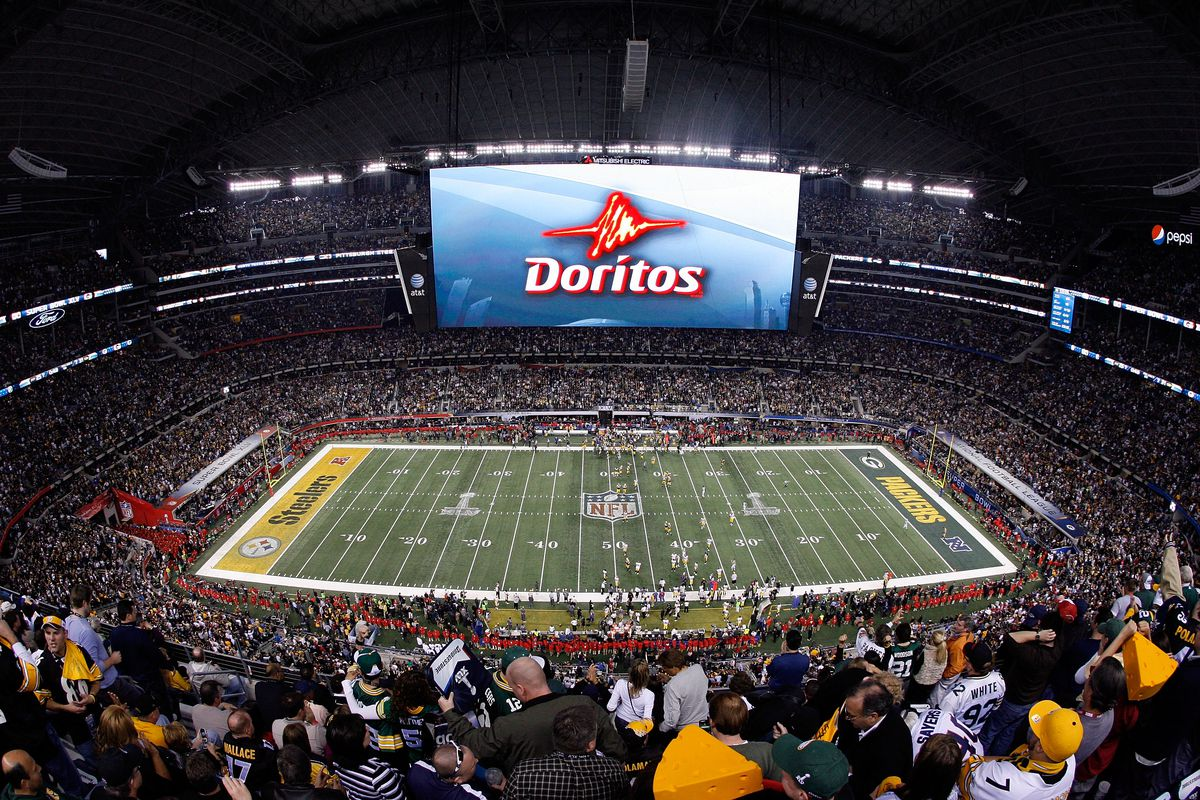
\includegraphics{https://raw.githubusercontent.com/mgino11/Super_Bowl_Ads_Analisys/main/doritossupebowl.0.jpg}
\caption{Super Bowl}
\end{figure}

\begin{Shaded}
\begin{Highlighting}[]
\FunctionTok{url.show}\NormalTok{(}\StringTok{"https://projects.fivethirtyeight.com/super{-}bowl{-}ads/"}\NormalTok{)}
\end{Highlighting}
\end{Shaded}

\hypertarget{packages}{%
\subsubsection{Packages}\label{packages}}

\begin{Shaded}
\begin{Highlighting}[]
\CommentTok{\#Packages used}

\FunctionTok{library}\NormalTok{(tidytext)}
\FunctionTok{library}\NormalTok{(DT)}
\FunctionTok{library}\NormalTok{(tm)}
\end{Highlighting}
\end{Shaded}

\begin{verbatim}
## Loading required package: NLP
\end{verbatim}

\begin{Shaded}
\begin{Highlighting}[]
\FunctionTok{library}\NormalTok{(tidyverse)}
\end{Highlighting}
\end{Shaded}

\begin{verbatim}
## -- Attaching packages --------------------------------------- tidyverse 1.3.0 --
\end{verbatim}

\begin{verbatim}
## v ggplot2 3.3.3     v purrr   0.3.4
## v tibble  3.0.5     v dplyr   1.0.3
## v tidyr   1.1.2     v stringr 1.4.0
## v readr   1.4.0     v forcats 0.5.1
\end{verbatim}

\begin{verbatim}
## -- Conflicts ------------------------------------------ tidyverse_conflicts() --
## x ggplot2::annotate() masks NLP::annotate()
## x dplyr::filter()     masks stats::filter()
## x dplyr::lag()        masks stats::lag()
\end{verbatim}

\begin{Shaded}
\begin{Highlighting}[]
\FunctionTok{library}\NormalTok{(stringr)}
\FunctionTok{library}\NormalTok{(magrittr)}
\end{Highlighting}
\end{Shaded}

\begin{verbatim}
## 
## Attaching package: 'magrittr'
\end{verbatim}

\begin{verbatim}
## The following object is masked from 'package:purrr':
## 
##     set_names
\end{verbatim}

\begin{verbatim}
## The following object is masked from 'package:tidyr':
## 
##     extract
\end{verbatim}

\begin{Shaded}
\begin{Highlighting}[]
\FunctionTok{library}\NormalTok{(leaflet)}
\FunctionTok{library}\NormalTok{(ggplot2)}
\FunctionTok{library}\NormalTok{(dplyr)}
\FunctionTok{library}\NormalTok{(plotly)}
\end{Highlighting}
\end{Shaded}

\begin{verbatim}
## 
## Attaching package: 'plotly'
\end{verbatim}

\begin{verbatim}
## The following object is masked from 'package:ggplot2':
## 
##     last_plot
\end{verbatim}

\begin{verbatim}
## The following object is masked from 'package:stats':
## 
##     filter
\end{verbatim}

\begin{verbatim}
## The following object is masked from 'package:graphics':
## 
##     layout
\end{verbatim}

\begin{Shaded}
\begin{Highlighting}[]
\FunctionTok{library}\NormalTok{(forcats)}
\end{Highlighting}
\end{Shaded}

\hypertarget{data-exploration}{%
\subsubsection{1.- Data Exploration}\label{data-exploration}}

\hypertarget{section}{%
\paragraph{}\label{section}}

\hypertarget{summary}{%
\subparagraph{1.1 Summary}\label{summary}}

GITHUB - place the original .csv in a github Repository and have R read
from the link.

\begin{Shaded}
\begin{Highlighting}[]
\NormalTok{superbowl\_ads }\OtherTok{\textless{}{-}}\FunctionTok{read.csv}\NormalTok{(}\StringTok{"https://raw.githubusercontent.com/mgino11/Super\_Bowl\_Ads\_Analisys/main/HW\_1\_superbowl{-}ads.csv"}\NormalTok{)}

\FunctionTok{glimpse}\NormalTok{(superbowl\_ads)}
\end{Highlighting}
\end{Shaded}

\begin{verbatim}
## Rows: 244
## Columns: 11
## $ year                      <int> 2018, 2020, 2006, 2018, 2003, 2020, 2020,...
## $ brand                     <chr> "Toyota", "Bud Light", "Bud Light", "Hynu...
## $ superbowl_ads_dot_com_url <chr> "https://superbowl-ads.com/good-odds-toyo...
## $ youtube_url               <chr> "https://www.youtube.com/watch?v=zeBZvwYQ...
## $ funny                     <chr> "False", "True", "True", "False", "True",...
## $ show_product_quickly      <chr> "False", "True", "False", "True", "True",...
## $ patriotic                 <chr> "False", "False", "False", "False", "Fals...
## $ celebrity                 <chr> "False", "True", "False", "False", "False...
## $ danger                    <chr> "False", "True", "True", "False", "True",...
## $ animals                   <chr> "False", "False", "True", "False", "True"...
## $ use_sex                   <chr> "False", "False", "False", "False", "True...
\end{verbatim}

\hypertarget{counting-qualitative-data}{%
\subparagraph{1.2 Counting Qualitative
Data}\label{counting-qualitative-data}}

\hypertarget{brands---who-has-the-most-adds}{%
\paragraph{Brands - Who has the most
adds?}\label{brands---who-has-the-most-adds}}

\hypertarget{from-the-information-below-we-are-able-to-determine-that-the-brand-with-the-greatest-amount-of-ads-is-budlight-followed-by-budweiser-and-in-third-place-we-can-find-doritos.}{%
\subparagraph{From the information below we are able to determine that
the brand with the greatest amount of ads is Budlight, followed by
Budweiser and in third place we can Find
Doritos.}\label{from-the-information-below-we-are-able-to-determine-that-the-brand-with-the-greatest-amount-of-ads-is-budlight-followed-by-budweiser-and-in-third-place-we-can-find-doritos.}}

\begin{Shaded}
\begin{Highlighting}[]
\NormalTok{ superbowl\_ads }\SpecialCharTok{\%\textgreater{}\%}
  \FunctionTok{count}\NormalTok{(brand) }\SpecialCharTok{\%\textgreater{}\%}
  \FunctionTok{arrange}\NormalTok{(}\FunctionTok{desc}\NormalTok{(n))}
\end{Highlighting}
\end{Shaded}

\begin{verbatim}
##        brand  n
## 1  Bud Light 60
## 2  Budweiser 43
## 3    Doritos 25
## 4      Pepsi 25
## 5    Hynudai 22
## 6  Coca-Cola 21
## 7    E-Trade 13
## 8        Kia 13
## 9        NFL 11
## 10    Toyota 11
\end{verbatim}

\hypertarget{sex}{%
\paragraph{Sex}\label{sex}}

\hypertarget{how-many-times-a-brand-has-used-adds-associated-with-sex}{%
\subparagraph{How many times a brand has used adds associated with
sex?}\label{how-many-times-a-brand-has-used-adds-associated-with-sex}}

\begin{Shaded}
\begin{Highlighting}[]
\NormalTok{superbowl\_ads }\SpecialCharTok{\%\textgreater{}\%}
  \FunctionTok{count}\NormalTok{(use\_sex) }\SpecialCharTok{\%\textgreater{}\%}
  \FunctionTok{arrange}\NormalTok{(}\FunctionTok{desc}\NormalTok{(n))}
\end{Highlighting}
\end{Shaded}

\begin{verbatim}
##   use_sex   n
## 1   False 181
## 2    True  63
\end{verbatim}

\hypertarget{animals}{%
\paragraph{Animals}\label{animals}}

\hypertarget{how-many-times-a-brand-has-used-adds-associated-with-animals}{%
\subparagraph{How many times a brand has used adds associated with
animals?}\label{how-many-times-a-brand-has-used-adds-associated-with-animals}}

\begin{Shaded}
\begin{Highlighting}[]
\NormalTok{superbowl\_ads }\SpecialCharTok{\%\textgreater{}\%}
  \FunctionTok{count}\NormalTok{(animals) }\SpecialCharTok{\%\textgreater{}\%}
  \FunctionTok{arrange}\NormalTok{(}\FunctionTok{desc}\NormalTok{(n))}
\end{Highlighting}
\end{Shaded}

\begin{verbatim}
##   animals   n
## 1   False 155
## 2    True  89
\end{verbatim}

\hypertarget{funny}{%
\paragraph{Funny}\label{funny}}

\hypertarget{how-many-times-a-brand-has-used-adds-associated-with-comedy}{%
\subparagraph{How many times a brand has used adds associated with
comedy?}\label{how-many-times-a-brand-has-used-adds-associated-with-comedy}}

\begin{Shaded}
\begin{Highlighting}[]
\NormalTok{superbowl\_ads }\SpecialCharTok{\%\textgreater{}\%}
  \FunctionTok{count}\NormalTok{(funny) }\SpecialCharTok{\%\textgreater{}\%}
  \FunctionTok{arrange}\NormalTok{(}\FunctionTok{desc}\NormalTok{(n))}
\end{Highlighting}
\end{Shaded}

\begin{verbatim}
##   funny   n
## 1  True 168
## 2 False  76
\end{verbatim}

\hypertarget{section-1}{%
\paragraph*{}\label{section-1}}
\addcontentsline{toc}{paragraph}{}

\hypertarget{data-wrangling}{%
\subsubsection{2.- Data Wrangling}\label{data-wrangling}}

\hypertarget{section-2}{%
\subparagraph{}\label{section-2}}

2.1 Subsets

Subset1 - Superbowl\_ads\_use

We subset data in order to understand it better. Subset\_1 allows us to
see the a new data frame including variables like

\begin{itemize}
\tightlist
\item
  Year
\item
  Brand
\item
  Use\_sex
\item
  Animals
\item
  Funny
\item
  Celebrity
\end{itemize}

\begin{Shaded}
\begin{Highlighting}[]
\NormalTok{superbowl\_ads }\SpecialCharTok{\%\textgreater{}\%} \FunctionTok{select}\NormalTok{(year, brand, funny, celebrity, animals, use\_sex)}
\end{Highlighting}
\end{Shaded}

\begin{verbatim}
##     year     brand funny celebrity animals use_sex
## 1   2018    Toyota False     False   False   False
## 2   2020 Bud Light  True      True   False   False
## 3   2006 Bud Light  True     False    True   False
## 4   2018   Hynudai False     False   False   False
## 5   2003 Bud Light  True     False    True    True
## 6   2020    Toyota  True      True    True   False
## 7   2020 Coca-Cola  True      True    True   False
## 8   2020       Kia False      True   False   False
## 9   2020   Hynudai  True      True    True   False
## 10  2020 Budweiser False      True   False   False
## 11  2010   Hynudai False     False   False   False
## 12  2010 Bud Light  True     False   False    True
## 13  2007 Budweiser  True     False    True    True
## 14  2002 Budweiser False     False    True   False
## 15  2020       NFL False      True   False   False
## 16  2017       NFL False     False   False   False
## 17  2005 Bud Light  True     False    True    True
## 18  2009     Pepsi  True     False   False   False
## 19  2004 Bud Light  True     False    True    True
## 20  2020   Doritos  True      True    True   False
## 21  2007 Bud Light  True     False   False   False
## 22  2020     Pepsi False      True   False   False
## 23  2019   Hynudai  True      True   False   False
## 24  2009 Budweiser False     False    True   False
## 25  2011       Kia  True     False   False    True
## 26  2019   Doritos False      True   False   False
## 27  2019     Pepsi  True      True   False    True
## 28  2013   Hynudai  True     False    True   False
## 29  2019       NFL  True      True   False   False
## 30  2011 Coca-Cola False     False   False   False
## 31  2019     Pepsi  True      True   False   False
## 32  2016   Hynudai  True     False    True   False
## 33  2010 Bud Light  True     False   False   False
## 34  2000   E-Trade  True     False    True   False
## 35  2001 Bud Light  True     False    True   False
## 36  2018   Doritos  True      True   False   False
## 37  2001 Budweiser  True     False   False   False
## 38  2018 Coca-Cola False      True   False   False
## 39  2013   Hynudai False     False    True   False
## 40  2004     Pepsi  True     False    True   False
## 41  2018       Kia False      True   False   False
## 42  2018     Pepsi False      True   False   False
## 43  2018       NFL  True      True   False   False
## 44  2010   E-Trade  True     False   False   False
## 45  2017       NFL False      True   False   False
## 46  2000   E-Trade  True     False   False   False
## 47  2007   E-Trade  True     False   False   False
## 48  2000 Budweiser  True     False   False   False
## 49  2013   Doritos  True     False    True   False
## 50  2013 Budweiser False     False   False    True
## 51  2007   Doritos  True     False   False    True
## 52  2009 Budweiser  True     False    True   False
## 53  2012   E-Trade  True     False   False   False
## 54  2019 Bud Light  True     False   False   False
## 55  2017       Kia  True      True    True   False
## 56  2007 Bud Light  True     False   False   False
## 57  2011 Bud Light  True     False    True   False
## 58  2016     Pepsi False      True   False   False
## 59  2009   Hynudai  True     False   False   False
## 60  2011 Coca-Cola  True     False    True   False
## 61  2016   Hynudai  True      True    True    True
## 62  2009   Doritos  True     False   False   False
## 63  2010   Doritos  True     False   False   False
## 64  2015   Doritos  True     False   False    True
## 65  2007 Coca-Cola False     False    True   False
## 66  2019    Toyota False     False   False   False
## 67  2002 Budweiser  True     False   False   False
## 68  2014 Coca-Cola  True     False   False   False
## 69  2004 Budweiser  True     False   False   False
## 70  2016 Coca-Cola  True      True   False   False
## 71  2015 Budweiser  True     False    True   False
## 72  2016   Hynudai  True      True   False   False
## 73  2001 Bud Light  True     False   False    True
## 74  2003 Bud Light  True     False   False   False
## 75  2000 Bud Light  True     False   False   False
## 76  2018 Coca-Cola False     False   False   False
## 77  2001     Pepsi  True     False   False    True
## 78  2014   Doritos  True     False    True   False
## 79  2016 Budweiser False      True   False   False
## 80  2004 Budweiser False     False    True   False
## 81  2015 Budweiser False     False    True   False
## 82  2016       Kia  True      True   False   False
## 83  2017 Budweiser False     False   False   False
## 84  2000 Budweiser  True     False    True   False
## 85  2009 Coca-Cola False     False    True   False
## 86  2015   Doritos  True     False    True   False
## 87  2004    Toyota  True     False   False   False
## 88  2016       NFL False      True   False   False
## 89  2017   Hynudai False     False   False   False
## 90  2012 Bud Light  True     False    True    True
## 91  2008 Budweiser False     False    True   False
## 92  2013   Hynudai  True     False    True   False
## 93  2010   Doritos  True     False   False   False
## 94  2016 Bud Light  True      True    True   False
## 95  2019    Toyota False     False   False   False
## 96  2009 Bud Light  True     False   False   False
## 97  2019 Budweiser False     False    True   False
## 98  2003 Bud Light  True     False   False    True
## 99  2019 Coca-Cola False     False    True   False
## 100 2012   Hynudai  True     False   False   False
## 101 2011   Hynudai  True     False   False   False
## 102 2015       Kia  True      True    True    True
## 103 2014 Budweiser False     False    True   False
## 104 2007 Bud Light  True     False   False   False
## 105 2008   Hynudai False     False   False   False
## 106 2010       NFL False     False   False   False
## 107 2005     Pepsi  True     False   False   False
## 108 2018 Budweiser False     False   False   False
## 109 2018 Bud Light  True     False    True   False
## 110 2004 Bud Light  True     False    True    True
## 111 2002 Budweiser  True     False   False   False
## 112 2006 Budweiser  True     False   False   False
## 113 2014 Bud Light False      True    True    True
## 114 2009 Coca-Cola  True     False    True   False
## 115 2014 Bud Light  True      True   False    True
## 116 2003 Bud Light  True     False   False    True
## 117 2014    Toyota  True      True    True   False
## 118 2009 Bud Light  True     False   False    True
## 119 2014       Kia False      True   False   False
## 120 2014   Hynudai  True      True   False    True
## 121 2013 Bud Light  True      True    True    True
## 122 2008 Bud Light  True     False   False   False
## 123 2003 Budweiser  True     False   False   False
## 124 2013 Bud Light  True      True   False   False
## 125 2011   Doritos  True     False    True   False
## 126 2005 Bud Light  True     False   False   False
## 127 2005 Budweiser  True     False    True   False
## 128 2014   Doritos  True     False    True   False
## 129 2008 Bud Light  True     False   False   False
## 130 2012     Pepsi False      True   False   False
## 131 2012   Doritos  True     False    True   False
## 132 2012    Toyota  True     False    True    True
## 133 2016   Doritos  True     False   False   False
## 134 2002 Bud Light  True     False    True    True
## 135 2002 Bud Light  True     False   False   False
## 136 2013   E-Trade  True     False    True   False
## 137 2008 Bud Light  True     False    True   False
## 138 2012 Coca-Cola False     False    True   False
## 139 2004     Pepsi  True     False   False   False
## 140 2010   Doritos  True     False    True   False
## 141 2012       Kia  True      True   False    True
## 142 2012       NFL False      True   False   False
## 143 2005 Bud Light  True     False   False    True
## 144 2010   Hynudai False      True   False   False
## 145 2004 Bud Light  True     False   False   False
## 146 2008 Bud Light  True     False   False    True
## 147 2016    Toyota  True     False   False   False
## 148 2006 Bud Light  True     False   False   False
## 149 2007 Coca-Cola False     False    True   False
## 150 2007 Budweiser False     False    True   False
## 151 2013   Doritos  True     False   False   False
## 152 2010 Bud Light  True      True   False   False
## 153 2009   Doritos  True     False    True    True
## 154 2009 Coca-Cola  True      True   False   False
## 155 2009     Pepsi False      True   False   False
## 156 2001   E-Trade False     False    True   False
## 157 2018 Bud Light  True     False    True   False
## 158 2015   Doritos  True     False   False    True
## 159 2010       Kia  True     False    True    True
## 160 2008   Doritos  True     False   False   False
## 161 2012 Coca-Cola False     False    True   False
## 162 2011   Hynudai False     False    True   False
## 163 2008 Coca-Cola  True      True   False   False
## 164 2000 Bud Light  True     False    True    True
## 165 2019       Kia False     False    True   False
## 166 2002 Bud Light  True     False   False    True
## 167 2013       Kia  True     False    True    True
## 168 2008     Pepsi  True      True   False    True
## 169 2019 Bud Light  True     False   False   False
## 170 2011   Hynudai False     False   False   False
## 171 2008 Bud Light  True      True   False    True
## 172 2008 Bud Light  True      True   False    True
## 173 2010   E-Trade  True     False   False    True
## 174 2013 Budweiser False     False   False    True
## 175 2001     Pepsi  True     False   False    True
## 176 2018 Coca-Cola False     False   False    True
## 177 2003 Bud Light  True     False   False   False
## 178 2011     Pepsi  True     False   False    True
## 179 2018   E-Trade  True     False   False    True
## 180 2016 Budweiser False     False    True   False
## 181 2008 Coca-Cola  True      True    True   False
## 182 2013       Kia  True     False   False    True
## 183 2014 Coca-Cola False     False    True   False
## 184 2012 Budweiser False     False    True   False
## 185 2004 Bud Light  True     False    True   False
## 186 2007 Bud Light  True      True   False   False
## 187 2007 Budweiser False      True   False   False
## 188 2019       Kia False     False   False   False
## 189 2002 Budweiser  True     False   False    True
## 190 2010   E-Trade  True     False   False   False
## 191 2003 Bud Light  True     False   False   False
## 192 2018    Toyota  True     False   False   False
## 193 2003 Budweiser  True     False    True   False
## 194 2013 Budweiser False     False    True   False
## 195 2010 Budweiser  True     False    True   False
## 196 2003 Bud Light  True     False    True   False
## 197 2002   E-Trade  True     False    True    True
## 198 2006 Budweiser  True     False   False   False
## 199 2012 Coca-Cola False     False    True   False
## 200 2019 Bud Light  True     False   False   False
## 201 2007    Toyota False     False   False   False
## 202 2014   Hynudai  True     False   False    True
## 203 2006     Pepsi  True      True   False   False
## 204 2006     Pepsi  True      True   False    True
## 205 2015     Pepsi False     False    True   False
## 206 2012 Bud Light False     False   False   False
## 207 2009   Doritos  True     False   False   False
## 208 2006 Budweiser  True     False    True    True
## 209 2014 Bud Light False     False   False   False
## 210 2005     Pepsi  True      True   False    True
## 211 2005 Bud Light  True      True    True    True
## 212 2007 Bud Light  True     False    True   False
## 213 2005     Pepsi  True      True   False    True
## 214 2015 Budweiser False     False    True   False
## 215 2019 Bud Light  True     False    True   False
## 216 2004 Bud Light  True      True   False    True
## 217 2003 Budweiser  True     False   False    True
## 218 2009   E-Trade  True     False   False   False
## 219 2013     Pepsi  True     False   False    True
## 220 2004 Budweiser  True      True    True    True
## 221 2009   Hynudai False     False   False   False
## 222 2014 Budweiser False     False    True   False
## 223 2003     Pepsi  True      True   False   False
## 224 2015 Coca-Cola False     False   False   False
## 225 2003       NFL False      True   False   False
## 226 2012   Doritos  True     False   False   False
## 227 2002     Pepsi False      True   False    True
## 228 2002 Bud Light  True      True   False    True
## 229 2000 Budweiser  True     False   False   False
## 230 2001 Bud Light  True      True   False    True
## 231 2013   Hynudai False     False   False   False
## 232 2015    Toyota False     False   False   False
## 233 2000 Budweiser  True     False    True   False
## 234 2001   Doritos  True      True   False    True
## 235 2016   Doritos  True     False    True   False
## 236 2008 Bud Light  True     False   False   False
## 237 2007   Doritos  True     False   False    True
## 238 2001       NFL False      True   False   False
## 239 2001     Pepsi  True      True    True    True
## 240 2014       NFL False     False   False   False
## 241 2012 Budweiser False     False    True    True
## 242 2001     Pepsi  True      True   False   False
## 243 2001   E-Trade  True     False   False   False
## 244 2001 Budweiser False      True   False   False
\end{verbatim}

\begin{Shaded}
\begin{Highlighting}[]
\FunctionTok{head}\NormalTok{(superbowl\_ads)}
\end{Highlighting}
\end{Shaded}

\begin{verbatim}
##   year     brand
## 1 2018    Toyota
## 2 2020 Bud Light
## 3 2006 Bud Light
## 4 2018   Hynudai
## 5 2003 Bud Light
## 6 2020    Toyota
##                                              superbowl_ads_dot_com_url
## 1                          https://superbowl-ads.com/good-odds-toyota/
## 2 https://superbowl-ads.com/2020-bud-light-seltzer-inside-posts-brain/
## 3                https://superbowl-ads.com/2006-bud-light-bear-attack/
## 4  https://superbowl-ads.com/hope-detector-nfl-super-bowl-lii-hyundai/
## 5                https://superbowl-ads.com/2003-bud-light-hermit-crab/
## 6 https://superbowl-ads.com/2020-toyota-go-places-with-cobie-smulders/
##                                   youtube_url funny show_product_quickly
## 1 https://www.youtube.com/watch?v=zeBZvwYQ-hA False                False
## 2 https://www.youtube.com/watch?v=nbbp0VW7z8w  True                 True
## 3 https://www.youtube.com/watch?v=yk0MQD5YgV8  True                False
## 4 https://www.youtube.com/watch?v=lNPccrGk77A False                 True
## 5 https://www.youtube.com/watch?v=ovQYgnXHooY  True                 True
## 6 https://www.youtube.com/watch?v=f34Ji70u3nk  True                 True
##   patriotic celebrity danger animals use_sex
## 1     False     False  False   False   False
## 2     False      True   True   False   False
## 3     False     False   True    True   False
## 4     False     False  False   False   False
## 5     False     False   True    True    True
## 6     False      True   True    True   False
\end{verbatim}

create data frame using Tibble

\begin{Shaded}
\begin{Highlighting}[]
\NormalTok{superbowl\_ads2 }\OtherTok{\textless{}{-}} \FunctionTok{as\_tibble}\NormalTok{(superbowl\_ads)}
\FunctionTok{colnames}\NormalTok{(superbowl\_ads2)}
\end{Highlighting}
\end{Shaded}

\begin{verbatim}
##  [1] "year"                      "brand"                    
##  [3] "superbowl_ads_dot_com_url" "youtube_url"              
##  [5] "funny"                     "show_product_quickly"     
##  [7] "patriotic"                 "celebrity"                
##  [9] "danger"                    "animals"                  
## [11] "use_sex"
\end{verbatim}

Factor \$ Levels

Subset\_1 = superbowl\_ads2

In order to understand Categorical Data we need to use Levels and
factors. The package used for this task is forcats

\begin{Shaded}
\begin{Highlighting}[]
\FunctionTok{glimpse}\NormalTok{(superbowl\_ads2)}
\end{Highlighting}
\end{Shaded}

\begin{verbatim}
## Rows: 244
## Columns: 11
## $ year                      <int> 2018, 2020, 2006, 2018, 2003, 2020, 2020,...
## $ brand                     <chr> "Toyota", "Bud Light", "Bud Light", "Hynu...
## $ superbowl_ads_dot_com_url <chr> "https://superbowl-ads.com/good-odds-toyo...
## $ youtube_url               <chr> "https://www.youtube.com/watch?v=zeBZvwYQ...
## $ funny                     <chr> "False", "True", "True", "False", "True",...
## $ show_product_quickly      <chr> "False", "True", "False", "True", "True",...
## $ patriotic                 <chr> "False", "False", "False", "False", "Fals...
## $ celebrity                 <chr> "False", "True", "False", "False", "False...
## $ danger                    <chr> "False", "True", "True", "False", "True",...
## $ animals                   <chr> "False", "False", "True", "False", "True"...
## $ use_sex                   <chr> "False", "False", "False", "False", "True...
\end{verbatim}

\begin{Shaded}
\begin{Highlighting}[]
\NormalTok{superbowl\_ads2 }\SpecialCharTok{\%\textgreater{}\%}
  \FunctionTok{mutate}\NormalTok{(}\AttributeTok{funny =} \FunctionTok{fct\_lump}\NormalTok{(funny, }\AttributeTok{n =} \DecValTok{50}\NormalTok{)) }\SpecialCharTok{\%\textgreater{}\%}
  \FunctionTok{count}\NormalTok{(funny)}
\end{Highlighting}
\end{Shaded}

\begin{verbatim}
## # A tibble: 2 x 2
##   funny     n
## * <fct> <int>
## 1 False    76
## 2 True    168
\end{verbatim}

Subset\_2

\begin{Shaded}
\begin{Highlighting}[]
\NormalTok{superbowl\_ads2 }\SpecialCharTok{\%\textgreater{}\%}
  \FunctionTok{count}\NormalTok{(use\_sex, celebrity)}
\end{Highlighting}
\end{Shaded}

\begin{verbatim}
## # A tibble: 4 x 3
##   use_sex celebrity     n
##   <chr>   <chr>     <int>
## 1 False   False       135
## 2 False   True         46
## 3 True    False        41
## 4 True    True         22
\end{verbatim}

\hypertarget{graphs}{%
\subsubsection{3.- Graphs}\label{graphs}}

\hypertarget{section-3}{%
\subparagraph{}\label{section-3}}

subset\_1

We want to interpret graphically the frequency of ads that use sex

\begin{Shaded}
\begin{Highlighting}[]
\FunctionTok{ggplot}\NormalTok{(superbowl\_ads2, }\FunctionTok{aes}\NormalTok{(}\AttributeTok{x =}\NormalTok{ use\_sex)) }\SpecialCharTok{+} 
  \FunctionTok{geom\_bar}\NormalTok{() }\SpecialCharTok{+}
  \FunctionTok{coord\_flip}\NormalTok{()}
\end{Highlighting}
\end{Shaded}

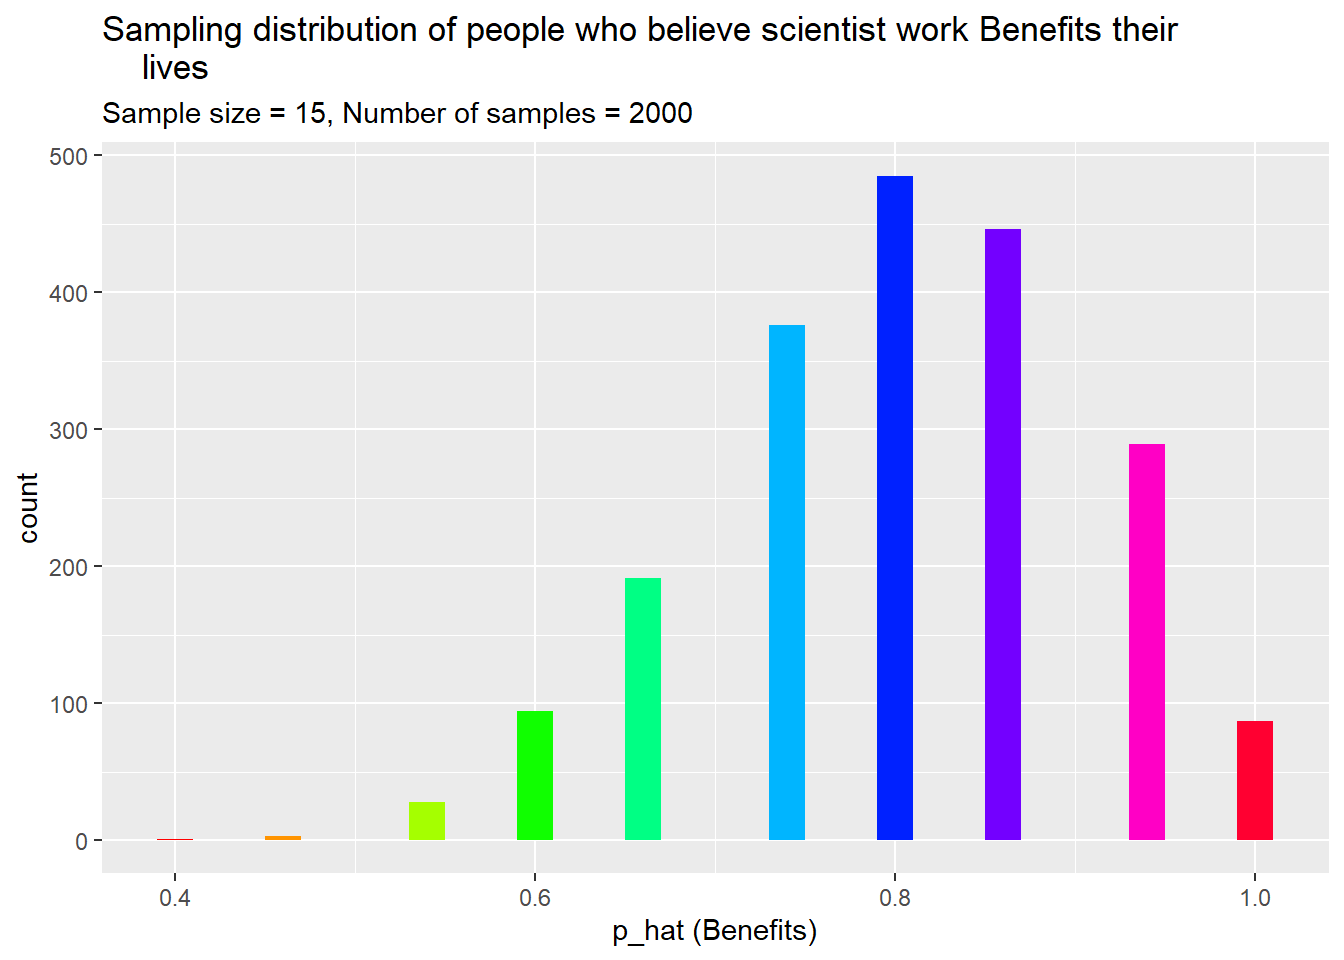
\includegraphics{DT607_HW_1_files/figure-latex/unnamed-chunk-13-1.pdf}

We want to interpret graphically the frequency of funny ads

\begin{Shaded}
\begin{Highlighting}[]
\FunctionTok{ggplot}\NormalTok{(superbowl\_ads2, }\FunctionTok{aes}\NormalTok{(}\AttributeTok{x =}\NormalTok{ funny)) }\SpecialCharTok{+} 
  \FunctionTok{geom\_bar}\NormalTok{() }\SpecialCharTok{+}
  \FunctionTok{coord\_flip}\NormalTok{()}
\end{Highlighting}
\end{Shaded}

\includegraphics{DT607_HW_1_files/figure-latex/unnamed-chunk-14-1.pdf}

We want to compare the use of sex in ads vs.~the use of comedy. We can
clearly see that comedy has been used more than sex.

\begin{Shaded}
\begin{Highlighting}[]
\FunctionTok{ggplot}\NormalTok{(superbowl\_ads2, }\FunctionTok{aes}\NormalTok{(}\AttributeTok{x =}\NormalTok{ funny, }\AttributeTok{fill =}\NormalTok{ use\_sex)) }\SpecialCharTok{+} 
  \FunctionTok{geom\_density}\NormalTok{(}\AttributeTok{col =} \ConstantTok{NA}\NormalTok{, }\AttributeTok{alpha =} \FloatTok{0.55}\NormalTok{)}
\end{Highlighting}
\end{Shaded}

\includegraphics{DT607_HW_1_files/figure-latex/unnamed-chunk-15-1.pdf}

\hypertarget{section-4}{%
\subparagraph*{}\label{section-4}}
\addcontentsline{toc}{subparagraph}{}

\hypertarget{conclusion}{%
\subsubsection{4.- Conclusion}\label{conclusion}}

\hypertarget{super-bowl-ads}{%
\paragraph{Super Bowl Ads}\label{super-bowl-ads}}

\hypertarget{sex-vs.-comedy}{%
\paragraph{SEX VS. COMEDY}\label{sex-vs.-comedy}}

\hypertarget{thanks-to-the-data-wrangling-and-graphs-we-can-now-understand-that-most-of-ads-we-see-have-more-inclination-for-the-use-of-sex-than-comedy.-and-since-we-determined-earlier---budlight-budweiser-doritos-are-the-brands-with-the-most-amunt-of-ads-over-the-years.}{%
\paragraph{Thanks to the Data Wrangling and Graphs we can now understand
that most of ads we see have more inclination for the use of sex than
comedy. And since we determined earlier - Budlight + Budweiser + Doritos
are the brands with the most amunt of ads over the
years.}\label{thanks-to-the-data-wrangling-and-graphs-we-can-now-understand-that-most-of-ads-we-see-have-more-inclination-for-the-use-of-sex-than-comedy.-and-since-we-determined-earlier---budlight-budweiser-doritos-are-the-brands-with-the-most-amunt-of-ads-over-the-years.}}

\begin{Shaded}
\begin{Highlighting}[]
\FunctionTok{ggplot}\NormalTok{(superbowl\_ads2, }\FunctionTok{aes}\NormalTok{(}\AttributeTok{x =}\NormalTok{ funny)) }\SpecialCharTok{+} 
  \FunctionTok{geom\_bar}\NormalTok{() }\SpecialCharTok{+}
  \FunctionTok{coord\_flip}\NormalTok{()}
\end{Highlighting}
\end{Shaded}

\includegraphics{DT607_HW_1_files/figure-latex/unnamed-chunk-16-1.pdf}

\begin{Shaded}
\begin{Highlighting}[]
\FunctionTok{ggplot}\NormalTok{(superbowl\_ads2, }\FunctionTok{aes}\NormalTok{(}\AttributeTok{x =}\NormalTok{ use\_sex)) }\SpecialCharTok{+} 
  \FunctionTok{geom\_bar}\NormalTok{() }\SpecialCharTok{+}
  \FunctionTok{coord\_flip}\NormalTok{()}
\end{Highlighting}
\end{Shaded}

\includegraphics{DT607_HW_1_files/figure-latex/unnamed-chunk-16-2.pdf}

\hypertarget{sex-vs.-funny-different-view}{%
\paragraph{SEX vs.~funny (different
view)}\label{sex-vs.-funny-different-view}}

\hypertarget{brands-seem-to-be-more-interested-in-pursuing-the-use-of-sex-in-ads-instead-of-comedy.}{%
\paragraph{Brands seem to be more interested in pursuing the use of sex
in ads instead of
comedy.}\label{brands-seem-to-be-more-interested-in-pursuing-the-use-of-sex-in-ads-instead-of-comedy.}}

\begin{Shaded}
\begin{Highlighting}[]
\FunctionTok{ggplot}\NormalTok{(superbowl\_ads2, }\FunctionTok{aes}\NormalTok{(}\AttributeTok{x =}\NormalTok{ funny, }\AttributeTok{fill =}\NormalTok{ use\_sex)) }\SpecialCharTok{+} 
  \FunctionTok{geom\_density}\NormalTok{(}\AttributeTok{col =} \ConstantTok{NA}\NormalTok{, }\AttributeTok{alpha =} \FloatTok{0.55}\NormalTok{)}
\end{Highlighting}
\end{Shaded}

\includegraphics{DT607_HW_1_files/figure-latex/unnamed-chunk-17-1.pdf}

\end{document}
